% gm-05-RightTriangles.tex

\documentclass[xcolor=dvipsnames]{beamer}

\usepackage{cancel}
\renewcommand{\CancelColor}{\color{red}}
\usepackage{graphicx}
\usepackage{wrapfig}
\usepackage{colortbl}
\usepackage{color}
\usepackage{alltt}
\renewcommand*{\thefootnote}{\fnsymbol{footnote}}
\definecolor{myblue}{rgb}{0.8,0.85,1}

\mode<presentation>
{
  \usetheme{Warsaw}
  \setbeamercovered{transparent}
}
% \usecolortheme[named=OliveGreen]{structure}
\setbeamertemplate{navigation symbols}{} 
\setbeamertemplate{blocks}[rounded][shadow=true] 

% this is for overlaying math symbols, see https://tex.stackexchange.com/questions/12895/overlay-symbol-with-another
\def\qeq{\mathrel{%
    \mathchoice{\QEQ}{\QEQ}{\scriptsize\QEQ}{\tiny\QEQ}%
}}
\def\QEQ{{%
    \setbox0\hbox{$\longrightarrow$}%
    \rlap{\hbox to \wd0{\hss/\hss}}\box0
  }}

\newcounter{expls}
\setcounter{expls}{0}
\newcommand{\beispiel}[1]{\refstepcounter{expls}\textbf{Example \arabic{expls}: #1.}}

\newcounter{exercise}
\setcounter{exercise}{0}
\newcommand{\ubung}[0]{\refstepcounter{exercise}\textbf{Exercise \arabic{exercise}: }}

\newif\ifBCITCourse
\BCITCoursetrue
% \BCITCoursefalse
\newif\ifWhichCourse
\WhichCoursetrue
\WhichCoursefalse
\ifBCITCourse
\ifWhichCourse
\newcommand{\CourseName}{Technical Mathematics for Food Technology}
\newcommand{\CourseNumber}{MATH 1441}
\newcommand{\CourseInst}{BCIT}
\else
\newcommand{\CourseName}{Technical Mathematics for Geomatics}
\newcommand{\CourseNumber}{MATH 1511}
\newcommand{\CourseInst}{BCIT}
\fi
\else
\newcommand{\CourseName}{Philosophy and Literature}
\newcommand{\CourseNumber}{PHIL 375}
\newcommand{\CourseInst}{UBC}
\fi

\title{Right Triangles}
\subtitle{{\CourseNumber}, BCIT}

\author{\CourseName}

\date{September 20, 2017}

\begin{document}

\begin{frame}
  \titlepage
\end{frame}

\begin{frame}
  \frametitle{What Is the Problem?}
A triangle has three sides and three angles that we can measure. 
  \begin{figure}[h]
    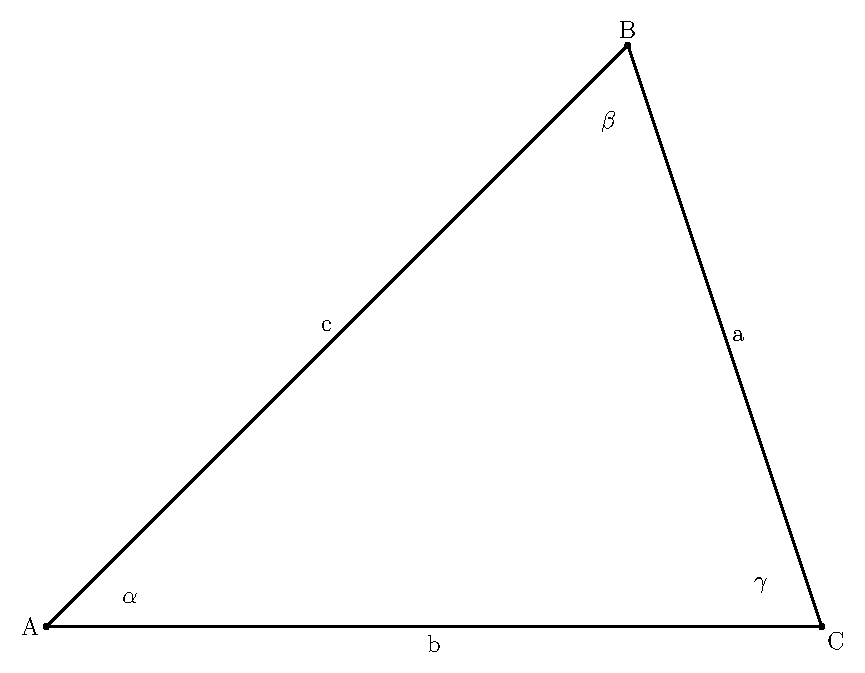
\includegraphics[scale=.3]{./acute.eps}
  \end{figure}
There are three vertices $A,B,C$, three sides $a,b,c$, and three
angles $\alpha,\beta,\gamma$. If three of them are given and three of
them are unknown, then how can we calculate (instead of measure) the
remaining three?
\end{frame}

\begin{frame}
  \frametitle{Towards a Solution: Right Triangles}
We can always divide any triangle into two (or fewer) right triangles.
Let's try to solve our problem first for right triangles.
  \begin{figure}[h]
    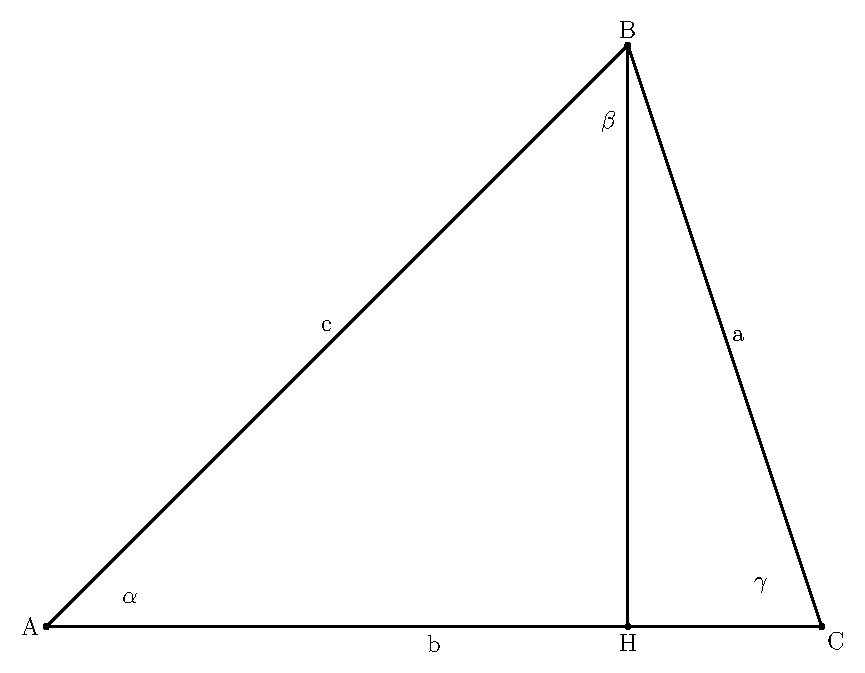
\includegraphics[scale=.3]{./acute-with-height.eps}
  \end{figure}
\end{frame}

\begin{frame}
  \frametitle{Bhaskara's Square}
  \begin{figure}[h]
    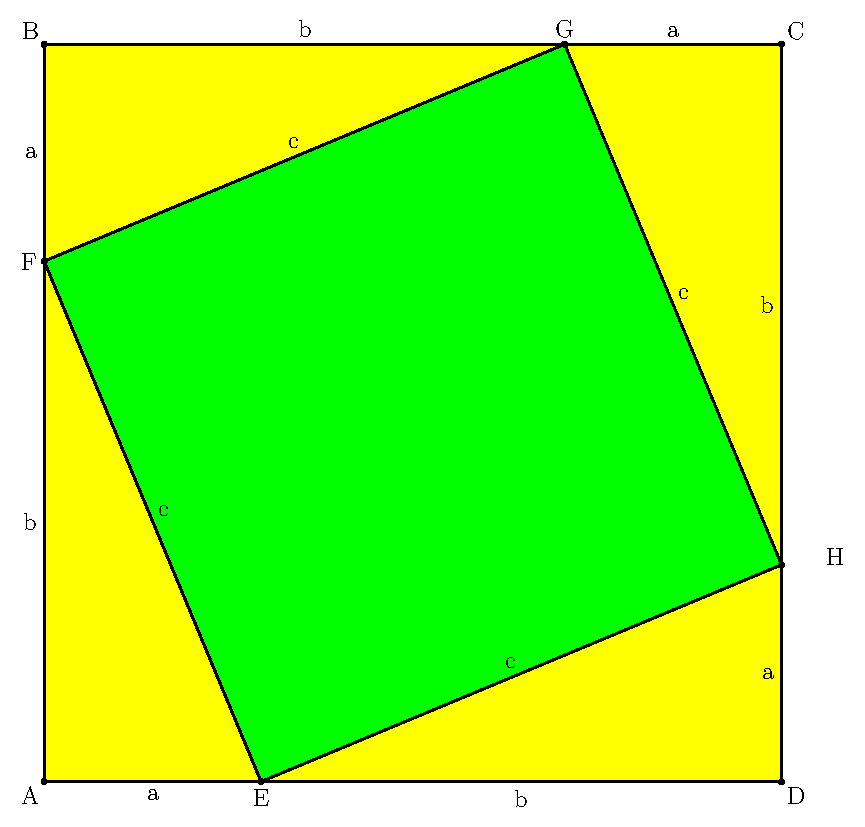
\includegraphics[scale=.5]{./pythagoras.eps}
  \end{figure}
\end{frame}

\begin{frame}
  \frametitle{Pythagorean Theorem}
  Calculate the area of the square in the diagram on the previous
  slide using two methods. Method 1: multiply the two sides of the
  large square (yellow and green). Method 2: add the area of the small
  square (green) to the four areas of the right triangles (yellow).
\begin{equation}
  \label{eq:aemoakee}
  A_{1}=(a+b)^{2}=a^{2}+2ab+b^{2}
\end{equation}
\begin{equation}
  \label{eq:eimelaij}
  A_{2}=c^{2}+2ab
\end{equation}
Since $A_{1}=A_{2}$, 
\begin{equation}
  \label{eq:eisheebi}
  c^{2}=a^{2}+b^{2}
\end{equation}
Consequently, given two sides of a right triangle, we can calculate
the length of the third side.
\end{frame}

\begin{frame}
  \frametitle{Definition of Sine and Cosine}
% 2016-12-16: I now recommend introducing the sine and cosine as the
% coordinates of points on the unit circle instead.
  Let $a,b,c$ be the sides of an arbitrary right triangle. Then
  consider the similar triangle $a',b',c'$, which has exactly the same
  angles but all sides are scaled by the factor $1/c$. This means that
  the side $c'$ has length 1 (we use the following notation: $c'=1$). 
\begin{equation}
  \label{eq:dioquite}
  \begin{array}{rcl}
    a'&=&\frac{a}{c} \\
    && \\
    b'&=&\frac{b}{c} \\
    && \\
    c'&=&1 \\
  \end{array}
\end{equation}
\end{frame}

\begin{frame}
  \frametitle{Definition of Sine and Cosine}
  Because $c'=1$, we can inscribe the right triangle in a unit circle
  as in the following diagram.
  \begin{figure}[h]
    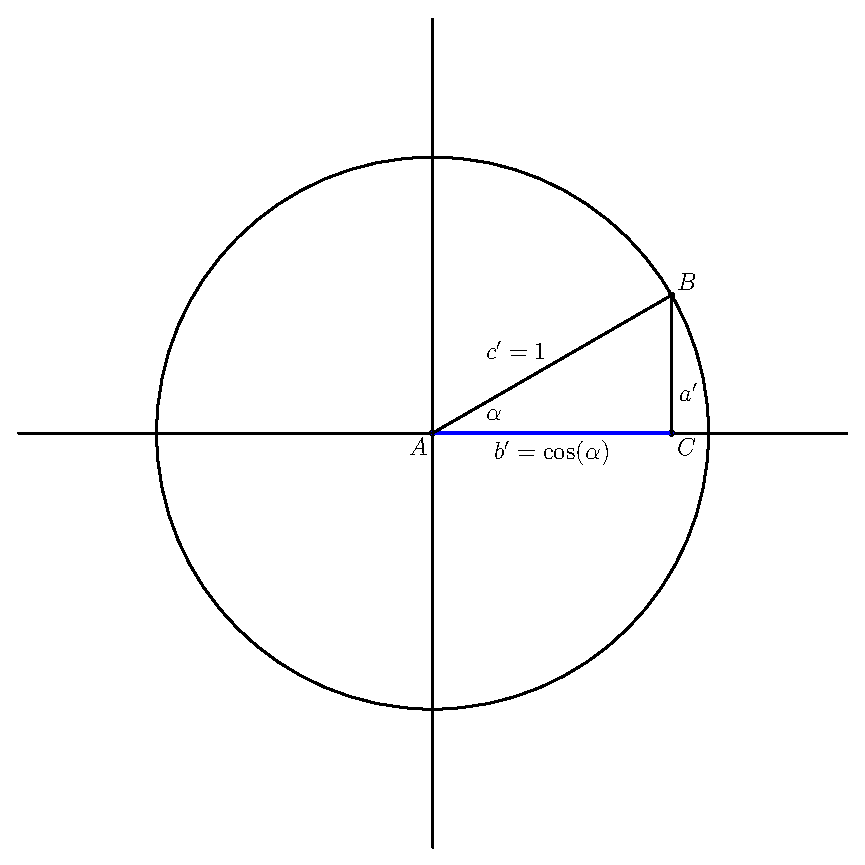
\includegraphics[scale=.5]{./cosine.eps}
  \end{figure}
\end{frame}

\begin{frame}
  \frametitle{Definition of Sine and Cosine}
Now define the cosine and sine of the angle $\alpha$ to be the
coordinates of the point $B$.
\begin{equation}
  \label{eq:eesiacha}
  \begin{array}{rcl}
    \sin(\alpha)&=&\frac{a}{c} \\
    && \\
    \cos(\alpha)&=&\frac{b}{c} \\
  \end{array}
\end{equation}
\end{frame}

\begin{frame}
  \frametitle{The Cosine Function}
  It is relatively easy to calculate the sine of an angle once you
  have the cosine and vice versa. We write $\cos^{2}\alpha$ as an
  abbreviation of $(\cos(\alpha))^{2}$.
  \begin{equation}
    \label{eq:aejeecob}
    \cos^{2}\alpha+\sin^{2}\alpha=1
  \end{equation}
  Consequently, it makes sense to focus on one of the two functions at
  first. We will focus on the cosine function.

  \bigskip
  
  How to calculate the cosine function for a given angle is still an
  open question. All we can see at this point is that it exists and
  that it is well-defined for angles between $0^{\circ}$ and
  $90^{\circ}$.
\end{frame}

\begin{frame}
  \frametitle{The Cosine Function}
  The following triangle illustrates why the cosine of
  $30^{\circ}$ is $\sqrt{3}/2$ and why the cosine of $60^{\circ}$ is
  $1/2$.
  \begin{figure}[h]
    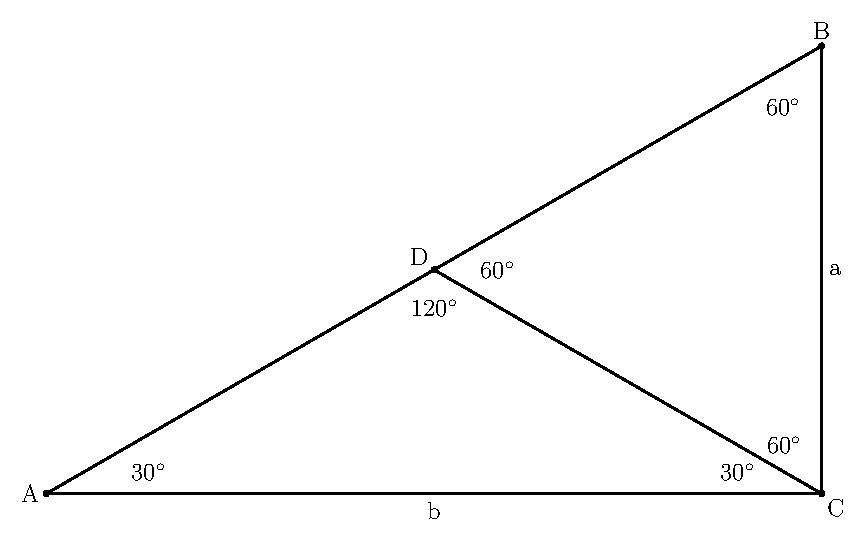
\includegraphics[scale=.5]{./thirty.eps}
  \end{figure}
\end{frame}

\begin{frame}
  \frametitle{The Cosine Function}
  If $\alpha=45^{\circ}$, then $a=b$. From the theorem of Pythagoras
  it follows that $\cos(45^{\circ})=\sqrt{2}/2$. Ptolemy's pentagram
  shows us that $\cos(36^{\circ})=0.80902$ (see Glen van Brummelen,
  ``Heavenly Mathematics,'' page 9). We now have enough data points to
  see the shape of the cosine curve between $0^{\circ}$ and
  $90^{\circ}$.
\end{frame}

\begin{frame}
  \frametitle{Ptolemy's Pentagram}
  Have a look at the diagram and find out why all angles in a
  pentagram add up to $540^{\circ}$. Notice that $\Delta{}ABC$ and
  $\Delta{}BHA$ are similar. Therefore (the length of segment $CH$ is
  1),
\begin{equation}
  \label{eq:ataicahd}
  \frac{1}{y+1}=\frac{y}{1}
\end{equation}
This is a quadratic equation with one positive solution,
\begin{equation}
  \label{eq:ziumahhi}
  y=\frac{1}{2}\left(\sqrt{5}-1\right)
\end{equation}
The length of segment $AC$ is $y+1$, but it's also twice the length of
segment $AF$. Therefore, the length of $AF$, which is
$cos(36^{\circ})$, is
\begin{equation}
  \label{eq:puuvahhi}
 cos(36^{\circ})=\frac{1}{4}\left(\sqrt{5}-1\right)+\frac{1}{2}=0.80902
\end{equation}
\end{frame}

\begin{frame}
  \frametitle{Ptolemy's Pentagram}
    \begin{figure}[h]
    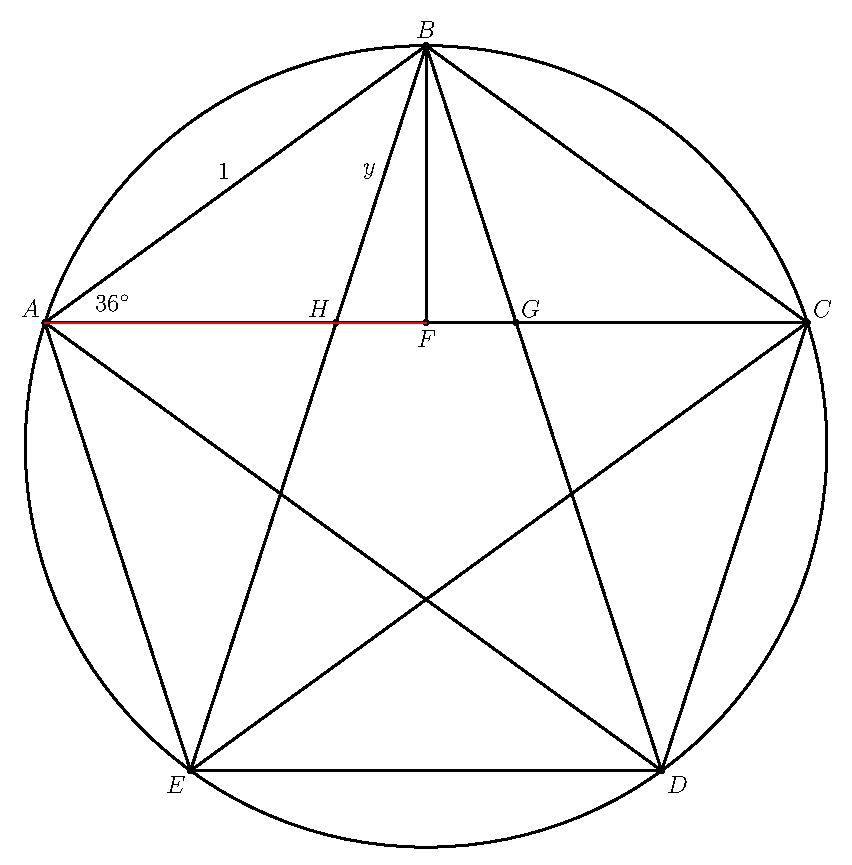
\includegraphics[scale=.6]{./ptolemy1.eps}
  \end{figure}
\end{frame}

\begin{frame}
  \frametitle{Ptolemy's Pentagram}
    \begin{figure}[h]
    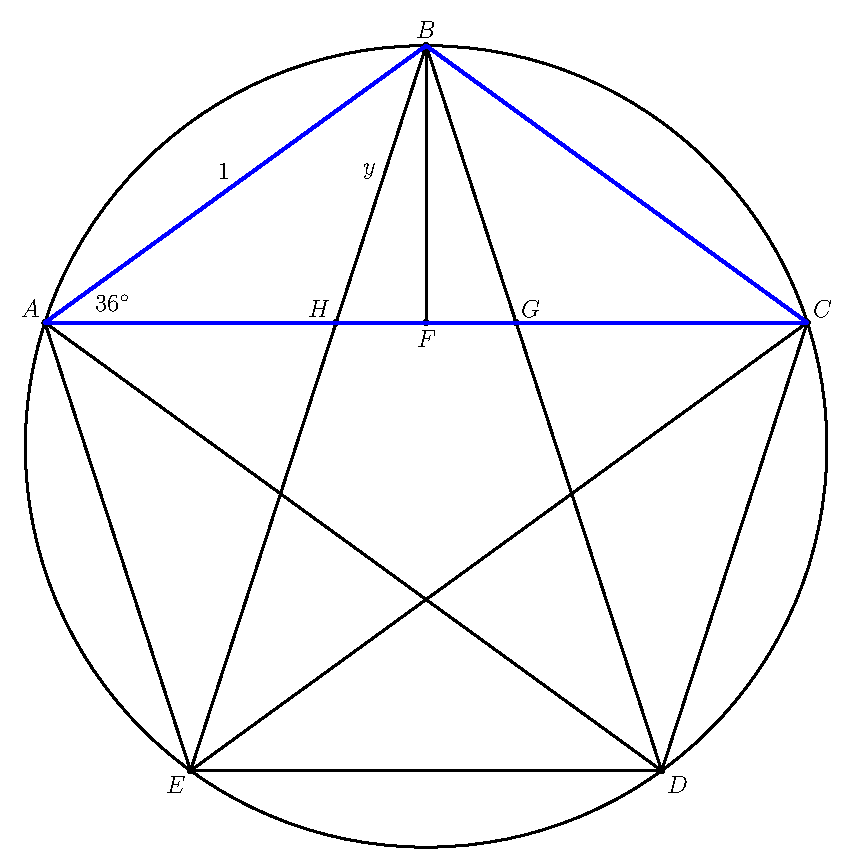
\includegraphics[scale=.6]{./ptolemy2.eps}
  \end{figure}
\end{frame}

\begin{frame}
  \frametitle{Ptolemy's Pentagram}
    \begin{figure}[h]
    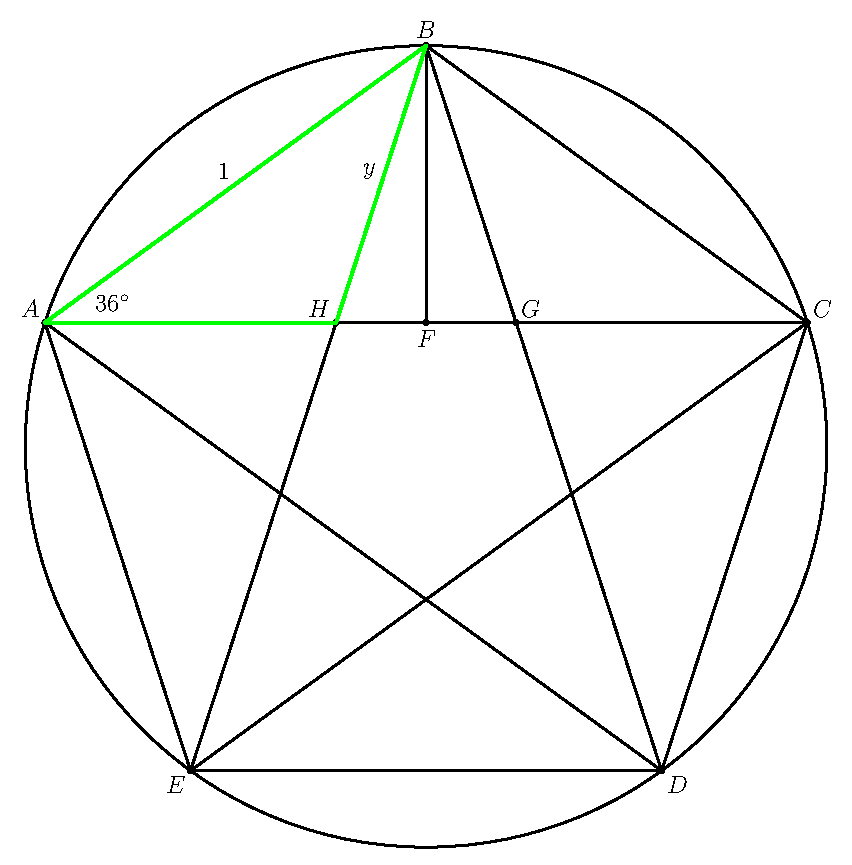
\includegraphics[scale=.6]{./ptolemy3.eps}
  \end{figure}
\end{frame}

\begin{frame}
  \frametitle{Ptolemy's Pentagram}
    \begin{figure}[h]
    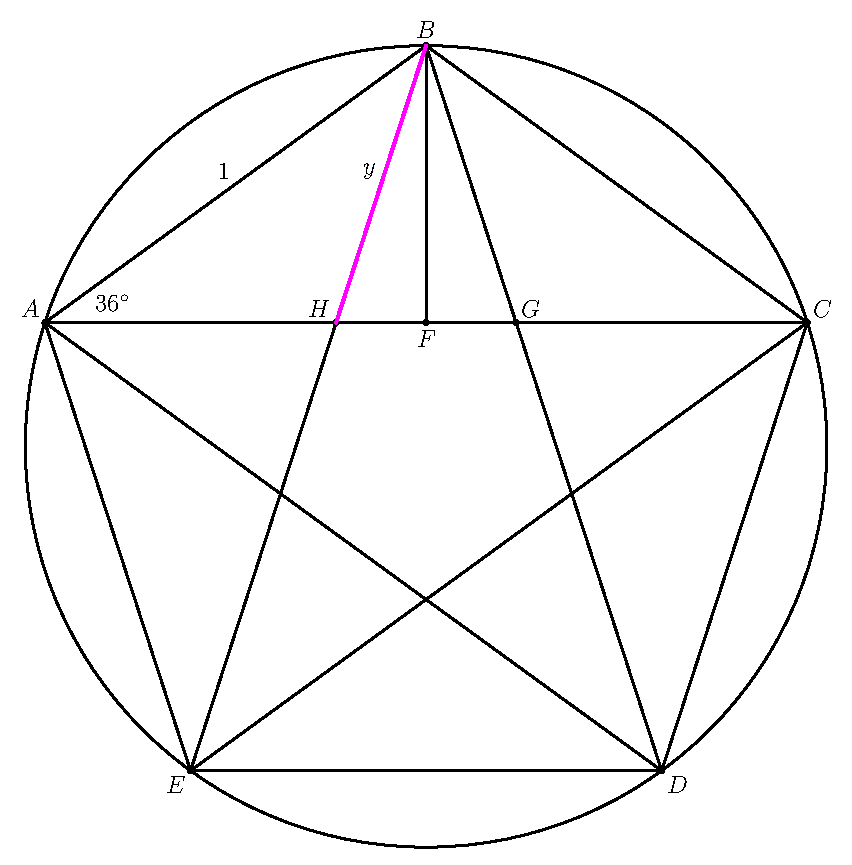
\includegraphics[scale=.6]{./ptolemy4.eps}
  \end{figure}
\end{frame}

\begin{frame}
  \frametitle{Ptolemy's Pentagram}
    \begin{figure}[h]
    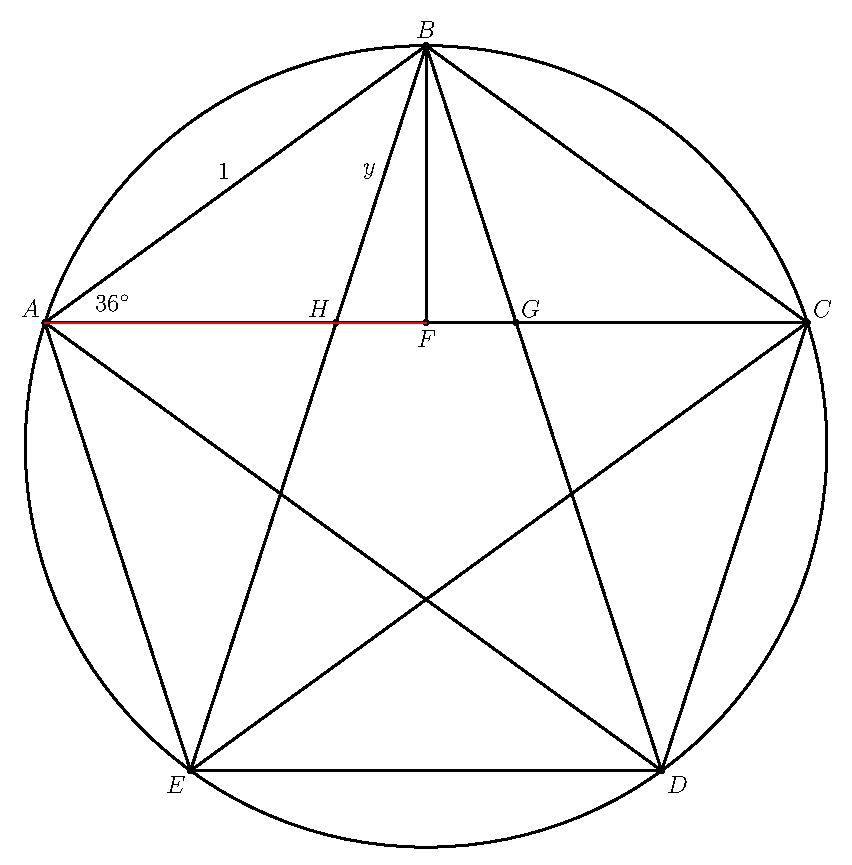
\includegraphics[scale=.6]{./ptolemy1.eps}
  \end{figure}
\end{frame}

\begin{frame}
  \frametitle{Reference Triangle}
  Let's have another look at this diagram, called the \alert{reference
  triangle}. 
  \begin{figure}[h]
    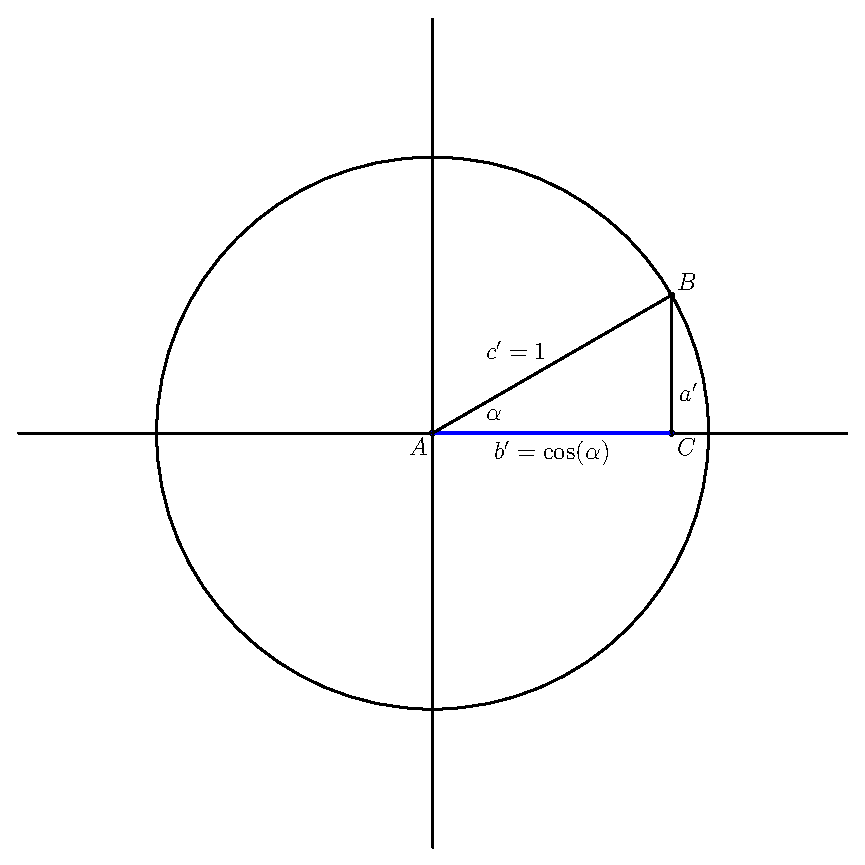
\includegraphics[scale=.5]{./cosine.eps}
  \end{figure}
\end{frame}

\begin{frame}
  \frametitle{The Cosine Function}
  Now let us define the cosine function for all angles (even negative
  ones). Think of $B$ going all the way around the circle, and think
  of $A$ as the origin of a coordinate system. The cosine and sine of
  $\alpha$ are defined as the coordinates of the point $B$, and the angle
  $\alpha$ can be anything from $-\infty$ to $\infty$. 
\end{frame}

\begin{frame}
  \frametitle{Radians}
  What kind of animal is $30^{\circ}$? It is a real number -- not the
  one you might expect. Just as $25\%$ is not the number 25, but the
  number $0.25$; and 3 quarters is not the number 3, but the number
  $0.75$.

  $30^{\circ}$ is not the number 30, but the number $\pi/6$. The
  \mbox{symbol $^{\circ}$} (pronounced ``degrees'') is equivalent to
  the factor $\pi/180$; just as the symbol $\%$ (pronounced
  ``percent'') is equivalent to the factor $1/100$, and a ``quarter'' is
  equivalent to the factor $1/4$.
  \begin{figure}[h]
    
\includegraphics[scale=.5]{./degreeradians.jpg}
  \end{figure}
\end{frame}

% \begin{frame}
%   \frametitle{The Sine Function}
% Define the sine function as follows,
% \begin{equation}
%   \label{eq:iedichoh}
% \sin\alpha=\sqrt{1-\cos^{2}\alpha}  
% \end{equation}
% In our diagram with the unit circle, the sine of $\alpha$ is just the
% side \alert{opposite} the angle $\alpha$, whereas the cosine of $\alpha$ is
% the side \alert{adjacent} to the angle $\alpha$. 

% Note that in this definition we have taken advantage of the following
% conventions in notation (both for cosine and sine),
% \begin{equation}
%   \label{eq:akohgaeg}
%   cos(\alpha)=\cos\alpha\mbox{ and }(\cos\alpha)^{2}=\cos^{2}\alpha
% \end{equation}
% \end{frame}

\begin{frame}
  \frametitle{Graph of Sine and Cosine Function}
From our definitions it follows that the graph of the sine and cosine
functions looks approximately like this,
  \begin{figure}[h]
    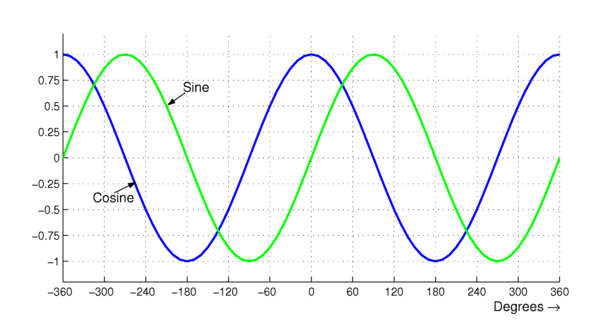
\includegraphics[scale=2]{./sinecosine.png}
  \end{figure}
\end{frame}

\begin{frame}
  \frametitle{Tangent Function}
Eventually, we will need a third function, the tangent function, which
is defined as
\begin{equation}
  \label{eq:bebiefee}
  \tan\alpha=\frac{\sin\alpha}{\cos\alpha}
\end{equation}
  \begin{figure}[h]
    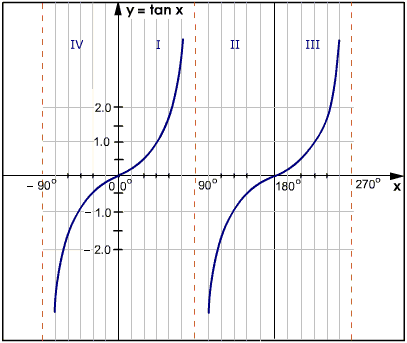
\includegraphics[scale=.5]{./tangent.png}
  \end{figure}
\end{frame}

\begin{frame}
  \frametitle{Problem of Three Missing Quantities}
  Let's see if we have made progress solving our problem of the three
  missing quantities. The way we have defined cosine and sine, it is
  apparent that for an arbitrary right triangle
  \begin{equation}
    \label{eq:eegahshi}
    \cos\alpha=\sin\beta=\frac{b}{c}
  \end{equation}
  \begin{equation}
    \label{eq:naxooshu}
    \sin\alpha=\cos\beta=\frac{a}{c}
  \end{equation}
  \begin{equation}
    \label{eq:hokoofai}
    \tan\alpha=\frac{a}{b}
  \end{equation}
  Together with $c^{2}=a^{2}+b^{2}$, (\ref{eq:eegahshi}),
  (\ref{eq:naxooshu}), and (\ref{eq:hokoofai}) are all the tools we
  need to solve any right triangle, i.e.\ find the missing three
  quantities if the remaining three (one of which is the right angle)
  are given.
\end{frame}

\begin{frame}
  \frametitle{SohCahToa}
A useful mnemonic device for the information on the last slide is
SOH-CAH-TOA, which stands for
\begin{equation}
  \label{eq:igeizeis}
  \sin\alpha=\frac{\mbox{opposite}}{\mbox{hypotenuse}}
\end{equation}
\begin{equation}
  \label{eq:eepheiku}
  \cos\alpha=\frac{\mbox{adjacent}}{\mbox{hypotenuse}}
\end{equation}
\begin{equation}
  \label{eq:eengiegh}
  \tan\alpha=\frac{\mbox{opposite}}{\mbox{adjacent}}
\end{equation}
\end{frame}

\begin{frame}
  \frametitle{Examples}
  \beispiel{Finding Three Missing Measurements} Let $ABC$ be a right
  triangle with a right angle at $C$, an angle $\alpha=39^{\circ}$,
  and a side $b=15$. Find the length of the side $a$.
  \begin{figure}[h]
    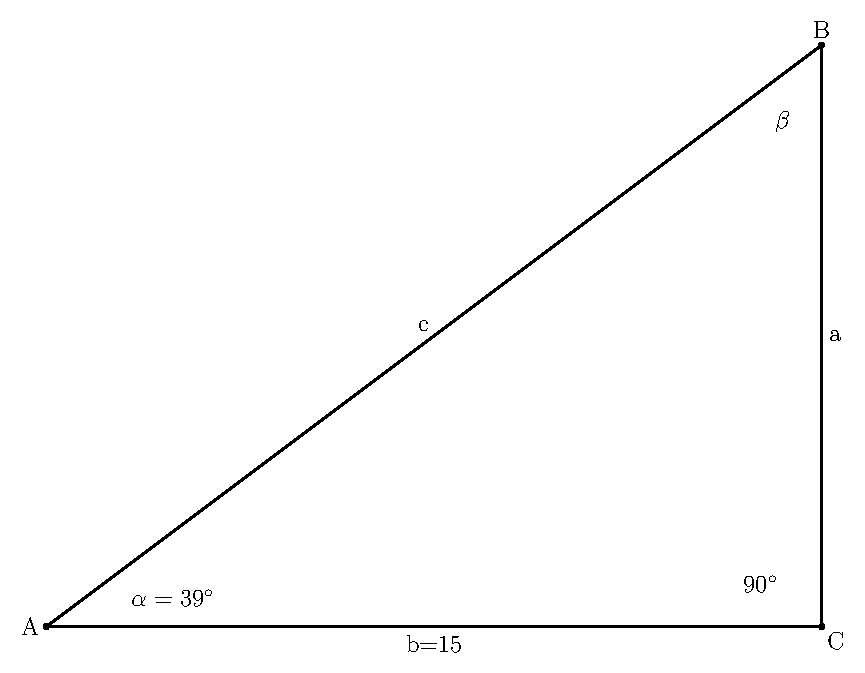
\includegraphics[scale=.5]{./rightex.eps}
  \end{figure}
\end{frame}

\begin{frame}
  \frametitle{Examples}
Use
\begin{equation}
  \label{eq:waipheik}
\tan(39^{\circ})=\frac{a}{15}
\end{equation}
and calculate
\begin{equation}
  \label{eq:aeceesah}
  a=15\tan(39^{\circ})\approx{}12.1468
\end{equation}
The length of the side $a\approx{}12.1468$.
\end{frame}

\begin{frame}
  \frametitle{Examples}
  \beispiel{Finding Three Missing Measurements} Let $ABC$ be a right
  triangle with a right angle at $C$, and sides $b=4,c=5$. Find the
  angle $\beta$.
  \begin{figure}[h]
    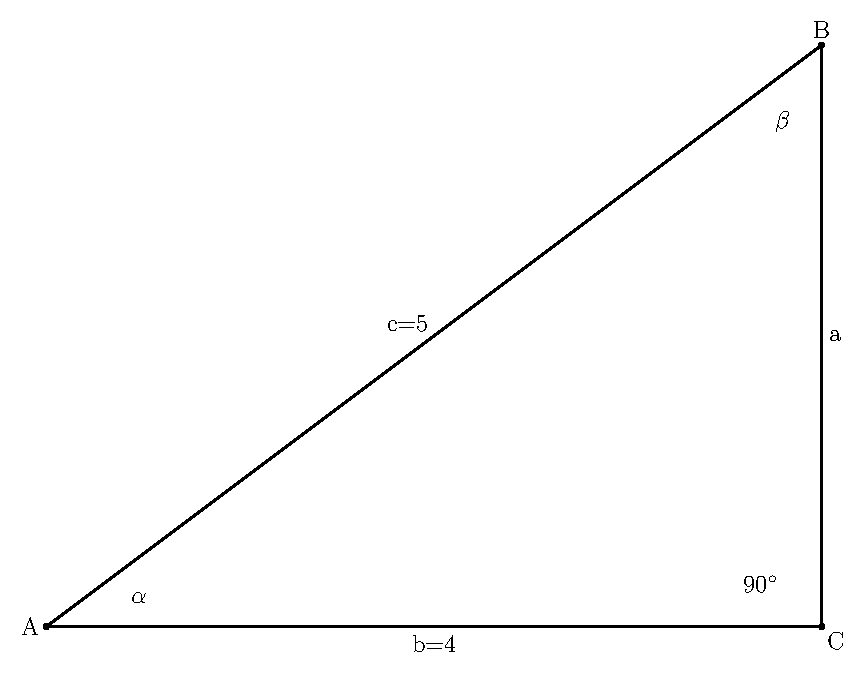
\includegraphics[scale=.5]{./rightey.eps}
  \end{figure}
\end{frame}

\begin{frame}
  \frametitle{Examples}
Use
\begin{equation}
  \label{eq:riechaev}
\sin\beta=\frac{4}{5}
\end{equation}
and calculate
\begin{equation}
  \label{eq:aithiegh}
  \beta=\arcsin\left(\frac{4}{5}\right)\approx{}53.130
\end{equation}
The angle $\beta\approx{}53.130$. Note that the arc sine function is
the inverse of the sine function, defined as
\begin{equation}
  \label{eq:thathuap}
  \arcsin(x)=\alpha\mbox{ only if }\sin\alpha=x
\end{equation}
There is also a corresponding arc cosine and arc tangent function.
\end{frame}

\begin{frame}
  \frametitle{Trigonometric Identities I}
  We ought not to be satisfied with what we have learned so far about
  solving the problem of the three missing quantities. The reason is
  that we have only defined the cosine function without giving any
  indication on how to calculate it. We have cosine values for
  $\alpha=0^{\circ},\alpha=30^{\circ},\alpha=36^{\circ},\alpha=45^{\circ},\alpha=60^{\circ},\alpha=90^{\circ}$,
  but what about other angles? A more generally satisfying answer to
  this question will need to come from the mathematical discipline of
  calculus, but in the meantime we can find more values for the cosine
  function by considering certain trigonometric identities. Here are
  some that are easy to derive from what we have already done,
  \begin{equation}
    \label{eq:aicheeho}
    \cos^{2}\alpha+\sin^{2}\alpha=1
  \end{equation}
  \begin{equation}
    \label{eq:ieshahko}
    \tan\alpha=\frac{\sin\alpha}{\cos\alpha}
  \end{equation}
\end{frame}

\begin{frame}
  \frametitle{Trigonometric Identities II}
Other trigonometric identities follow from careful consideration of
the reference triangle,
\begin{equation}
  \label{eq:iegaexah}
  \sin(-\alpha)=-\sin\alpha
\end{equation}
\begin{equation}
  \label{eq:gaijohra}
  \cos(-\alpha)=\cos\alpha
\end{equation}
\begin{equation}
  \label{eq:doajeigh}
  \tan(-\alpha)=-\tan\alpha
\end{equation}
and also,
\begin{equation}
  \label{eq:dieteipa}
  \sin(90^{\circ}-\alpha)=\cos\alpha
\end{equation}
\begin{equation}
  \label{eq:oepoodoh}
  \cos(90^{\circ}-\alpha)=\sin\alpha
\end{equation}
\begin{equation}
  \label{eq:aiwatong}
  \tan(90^{\circ}-\alpha)=\frac{1}{\tan\alpha}
\end{equation}
The last function, $\cot\alpha=\frac{1}{\tan\alpha}$ is also called
the cotangent function. The identities on this page are reflection
identities.
\end{frame}

\begin{frame}
  \frametitle{Trigonometric Identities III}
Here are some identities related to shifts and periodicity,
\begin{equation}
  \label{eq:owoofaiw}
  \sin(\alpha+90^{\circ})=\cos\alpha
\end{equation}
\begin{equation}
  \label{eq:ohbixiem}
  \cos(\alpha+90^{\circ})=-\sin\alpha
\end{equation}
\begin{equation}
  \label{eq:kaitohbu}
  \tan(\alpha+90^{\circ})=-\cot\alpha
\end{equation}
and also,
\begin{equation}
  \label{eq:jahpeexu}
  \sin(\alpha+180^{\circ})=-\sin\alpha
\end{equation}
\begin{equation}
  \label{eq:aephuemo}
  \cos(\alpha+180^{\circ})=-\cos\alpha
\end{equation}
\begin{equation}
  \label{eq:xaiyahcu}
  \tan(\alpha+180^{\circ})=\tan\alpha
\end{equation}
\begin{equation}
  \label{eq:aitahwae}
  \cot(\alpha+180^{\circ})=\cot\alpha
\end{equation}
All trigonometric functions repeat when an integer multiple of
$360^{\circ}$ is added, i.e.\
$\mbox{trigfun}(\alpha+k\cdot360^{\circ})=\mbox{trigfun}(\alpha)$.
\end{frame}

\begin{frame}
  \frametitle{Angle Sum Identities I}
  Here is a trigonometric identity that will help us find more cosine
  values, using what we have learned so far. Consider the following
  diagram.
  \begin{figure}[h]
    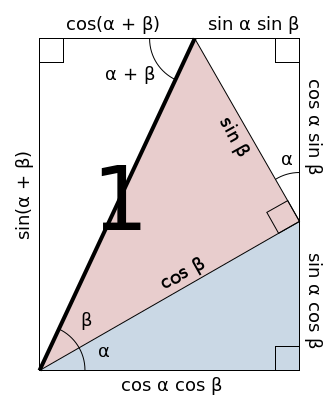
\includegraphics[scale=.45]{./anglesum.png}
  \end{figure}
\end{frame}

\begin{frame}
  \frametitle{Angle Sum Identities II}
From the diagram, we deduce
\begin{equation}
  \label{eq:eitaiquu}
  \sin(\alpha+\beta)=\sin\alpha\cos\beta+\cos\alpha\sin\beta
\end{equation}
\begin{equation}
  \label{eq:iasoojou}
  \cos(\alpha+\beta)=\cos\alpha\cos\beta-\sin\alpha\sin\beta
\end{equation}
This means we can calculate cosine values of all angles between
$0^{\circ}$ and $90^{\circ}$ that are divisible by three, for example
\begin{equation}
  \label{eq:uziajoch}
  \cos(6^{\circ})=\sin(84^{\circ})=\sin(30^{\circ}+54^{\circ})=\notag
\end{equation}
\begin{equation}
  \label{eq:chaevuer}
  \cos(30^{\circ})\sin(54^{\circ})+\cos(54^{\circ})\sin(30^{\circ})
\end{equation}
where
\begin{equation}
  \label{eq:puhahwie}
  \sin(54^{\circ})=\cos(36^{\circ})
\end{equation}
and
\begin{equation}
  \label{eq:chooteph}
  \cos(54^{\circ})=\sqrt{1-\sin^{2}(54^{\circ})}
\end{equation}
\end{frame}

\begin{frame}
  \frametitle{Double-Angle Formula}
  If $\alpha=\beta$, the angle sum identities give us the double-angle
  formulas
  \begin{equation}
    \label{eq:icuchodo}
    \sin(2\alpha)=2\cos\alpha\sin\alpha
  \end{equation}
  \begin{equation}
    \label{eq:woojahtu}
    \cos(2\alpha)=\cos^{2}\alpha-\sin^{2}\alpha
  \end{equation}
  Now we can calculate cosine values of angles that are not divisible
  by three and create a much more fine-grained web of values, even
  though we have no general formula how to calculate cosine values
  (this will have to wait until we learn calculus). For example
  \begin{equation}
    \label{eq:aoghaehu}
    \cos(10.5^{\circ})=\sqrt{\frac{\cos(21^{\circ})+1}{2}}
  \end{equation}
\end{frame}

\begin{frame}
  \frametitle{List of Cosines (and Sines)}
  % CosinesAndSines.ods
  \begin{figure}[h]
    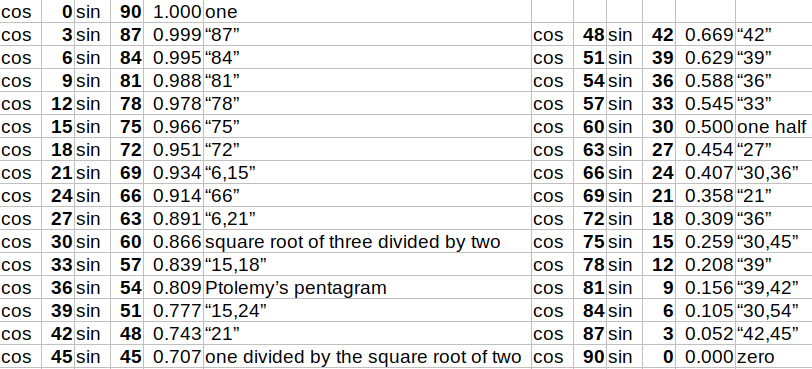
\includegraphics[scale=.4]{./SinCos2.png}
  \end{figure}
\end{frame}

\begin{frame}
  \frametitle{List of Cosines (and Sines)}
  % CosinesAndSines.ods
  \begin{figure}[h]
    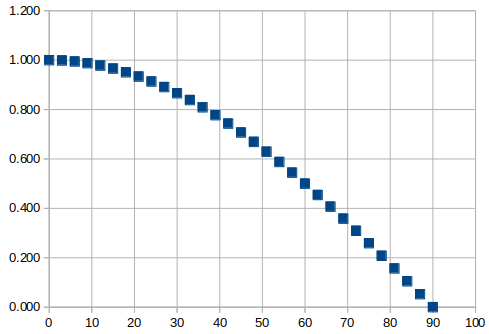
\includegraphics[scale=.6]{./SinCos1.png}
  \end{figure}
\end{frame}

\begin{frame}
  \frametitle{Solving Trigonometric Equations}
{\ubung} Solve the following trigonometric equations:
\begin{equation}
  \label{eq:vuagexai}
  \sin\vartheta+7=8
\end{equation}
\begin{equation}
  \label{eq:iiyiehah}
  \tan^{2}\vartheta-3=0
\end{equation}
\begin{equation}
  \label{eq:iehephoo}
  2\cos^{2}(\vartheta)-\sqrt{3}\cos\vartheta=0
\end{equation}
\begin{equation}
  \label{eq:yoopufae}
  \sin^{2}\vartheta+2\cos\vartheta=2
\end{equation}
\begin{equation}
  \label{eq:eewengah}
  \sin\vartheta=\sin(2\vartheta)
\end{equation}
\begin{equation}
  \label{eq:ooghiemu}
  \sin\vartheta+\cos\vartheta=1
\end{equation}
\end{frame}

\begin{frame}
  \frametitle{Astronomical Distances}
  The Greek mathematician Eratosthenes measured the circumference of
  the earth from the following observations. He noticed that on a
  certain day the sun shone directly down a deep well in Syene (modern
  Aswan). At the same time in Alexandria, 500 miles north (on the same
  meridian), the rays of the sun shone at an angle of 7.2$^{\circ}$ to the
  zenith. Use this information and the figure to find the radius and
  circumference of the earth. (The data used in this problem are
  more accurate than those available to Eratosthenes.)
\end{frame}

\begin{frame}
  \frametitle{Astronomical Distances}
  \begin{figure}[h]
    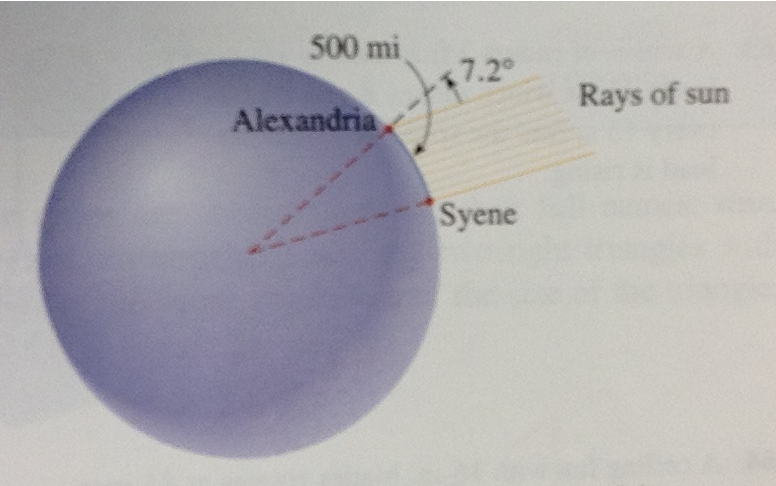
\includegraphics[scale=.4]{./eratosthenes.png}
  \end{figure}
\end{frame}

\begin{frame}
  \frametitle{Astronomical Distances}
  Here is a way to estimate the distance from the earth to the moon:
  When the moon is seen at its zenith at a point $A$ on the earth, it
  is observed to be at the horizon from point $B$ (see the figure).
  Point $A$ and $B$ are 6155 miles apart, and the radius of the earth
  is 3960 miles. Find the angle $\theta$ in degrees. Estimate the
  distance from point $A$ to the moon.
\end{frame}

\begin{frame}
  \frametitle{Astronomical Distances}
  \begin{figure}[h]
    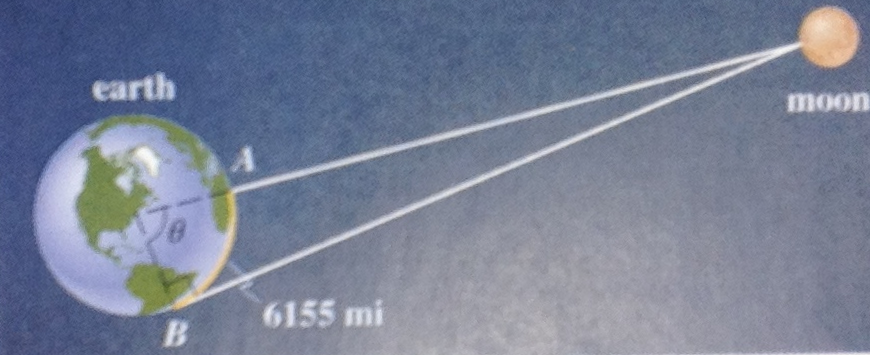
\includegraphics[scale=.35]{./earthmoon.png}
  \end{figure}
\end{frame}

\begin{frame}
  \frametitle{Astronomical Distances}
  When the moon is exactly half full, the earth, moon, and sun form a
  right angle (see the figure). At that time the angle formed by the
  sun, earth, and the moon is measured to be 89.85$^{\circ}$. If the
  distance from the earth to the moon is 240,000 miles, estimate the
  distance from the earth to the sun.
\end{frame}

\begin{frame}
  \frametitle{Astronomical Distances}
  \begin{figure}[h]
    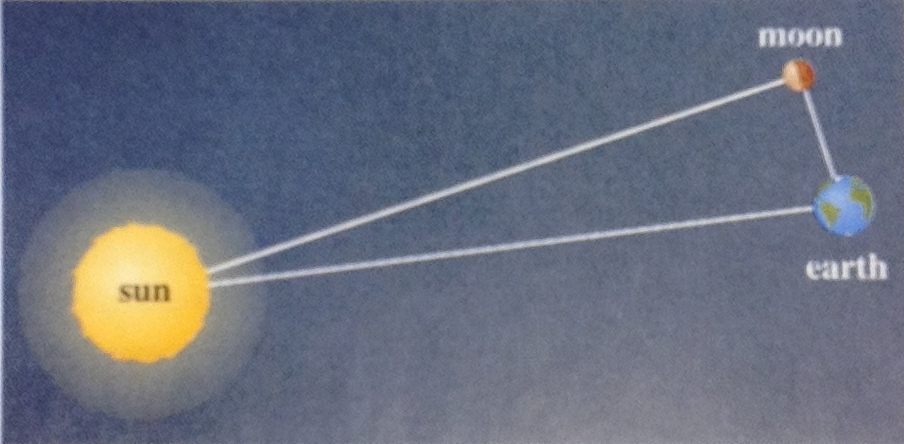
\includegraphics[scale=.35]{./earthsun.png}
  \end{figure}
\end{frame}

\begin{frame}
  \frametitle{Astronomical Distances}
  To find the distance to nearby stars, the method of parallax is
  used. The idea is to find a triangle with a star at one vertex and
  with the base as large as possible. To do this, the star is observed
  at two different times exactly 6 months apart, and its apparent
  change in position is recorded. From these two observations,
  $\angle{}E_{1}SE_{2}$ can be calculated. (The times are chosen so
  that $\angle{}E_{1}SE_{2}$ is as large as possible, which guarantees
  that $\angle{}E_{1}OS$ is 90°.) The angle $\angle{}E_{1}SO$ is
  called the \emph{parallax} of the star. Alpha Centauri, the star
  nearest the earth, has a parallax of $0.000211^{\circ}$. Estimate the
  distance to this star. (Take the distance from the earth to the sun
  to be $9.3\cdot{}10^{7}$ miles.)
\end{frame}
\begin{frame}
  \frametitle{Astronomical Distances}
  \begin{figure}[h]
    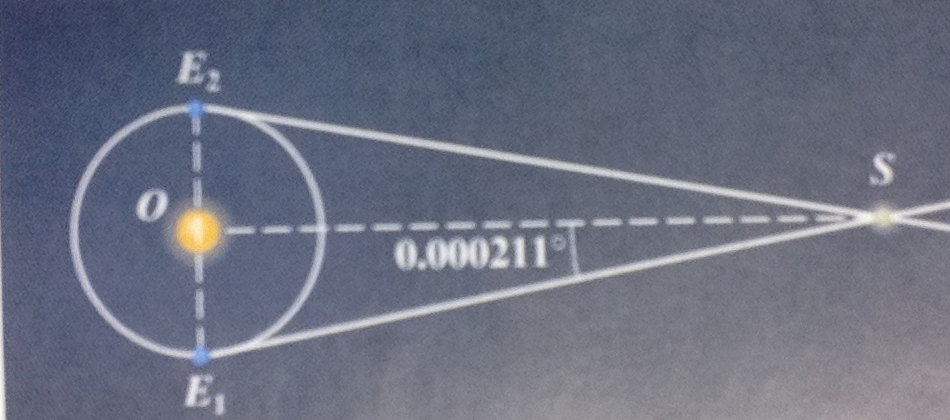
\includegraphics[scale=.35]{./parallax.png}
  \end{figure}
\end{frame}

\begin{frame}
  \frametitle{Exercises}
{\ubung} Calculate the remaining side/angle values. $a=23.453mm,b=15.791mm$.
  \begin{figure}[h]
    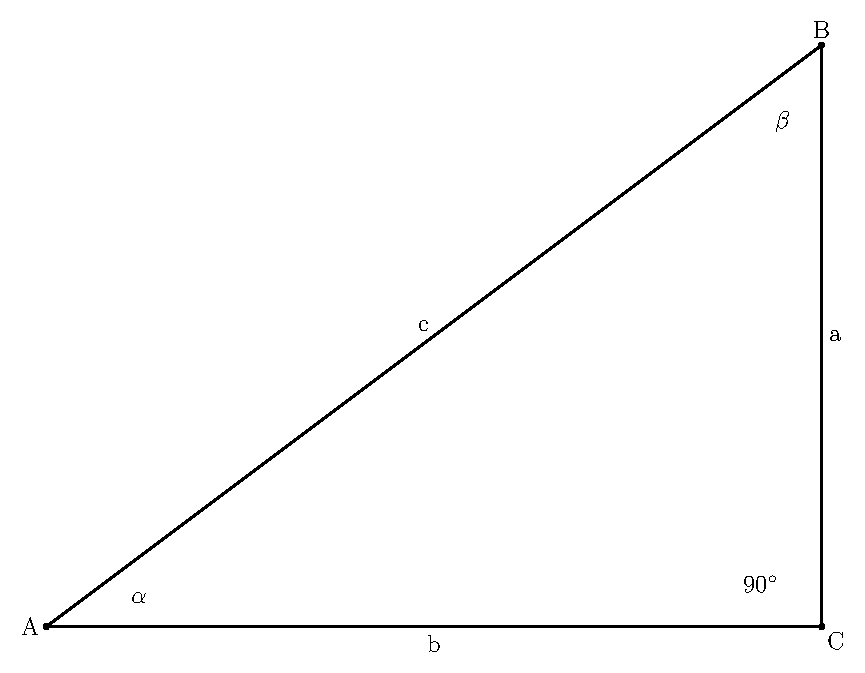
\includegraphics[scale=.3]{./right.eps}
  \end{figure}
\end{frame}

\begin{frame}
  \frametitle{Exercises}
{\ubung} Calculate the remaining side/angle values. $\beta=78^{\circ}34'12'',b=15.791m$.
  \begin{figure}[h]
    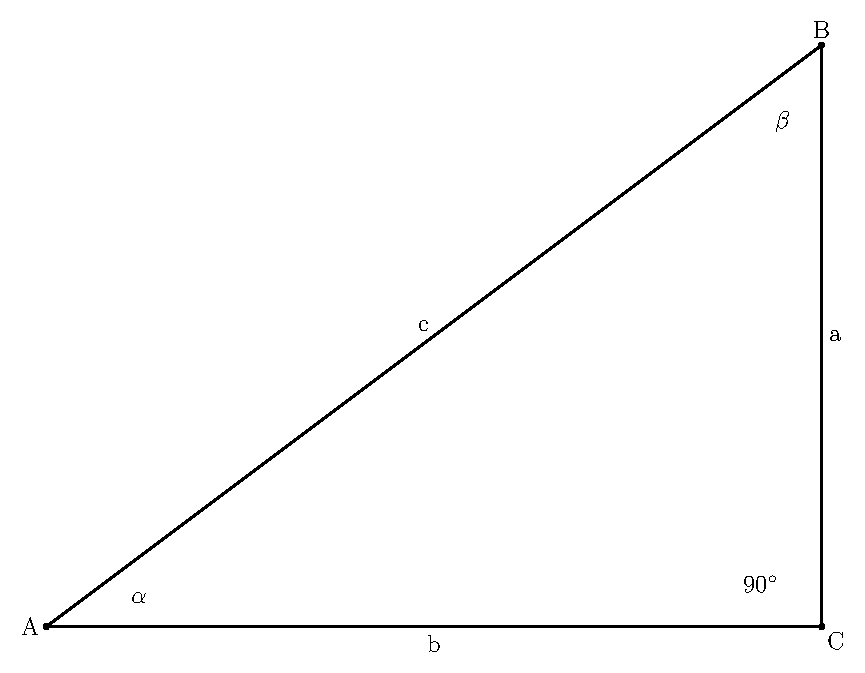
\includegraphics[scale=.3]{./right.eps}
  \end{figure}
\end{frame}

\begin{frame}
  \frametitle{Exercises}
{\ubung} Calculate the remaining side/angle values. $c=89.221m,a=75.791m$.
  \begin{figure}[h]
    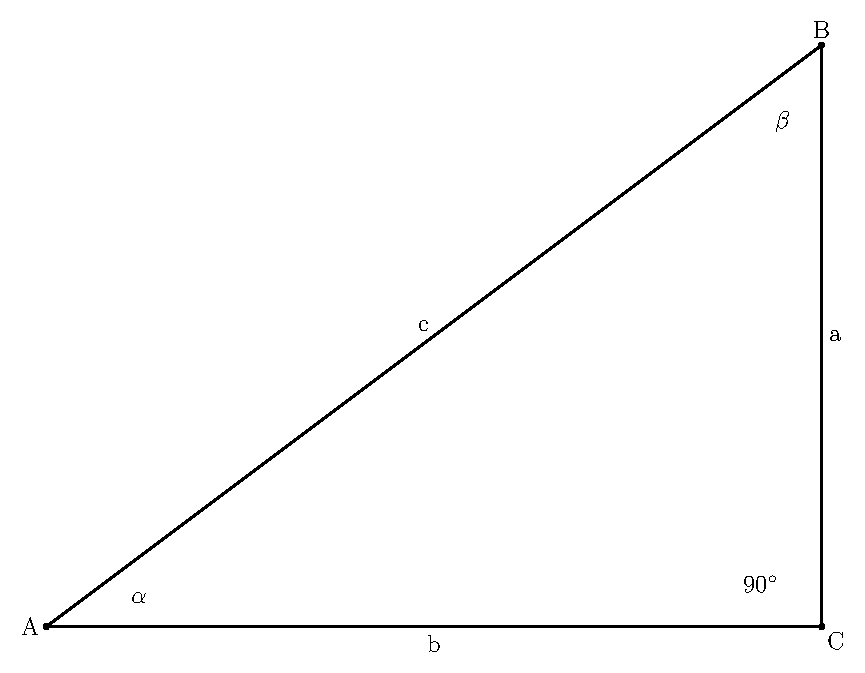
\includegraphics[scale=.3]{./right.eps}
  \end{figure}
\end{frame}

\begin{frame}
  \frametitle{Exercises}
{\ubung} Calculate the remaining side/angle values. $\alpha=24^{\circ}44'05'',c=12.998mm$.
  \begin{figure}[h]
    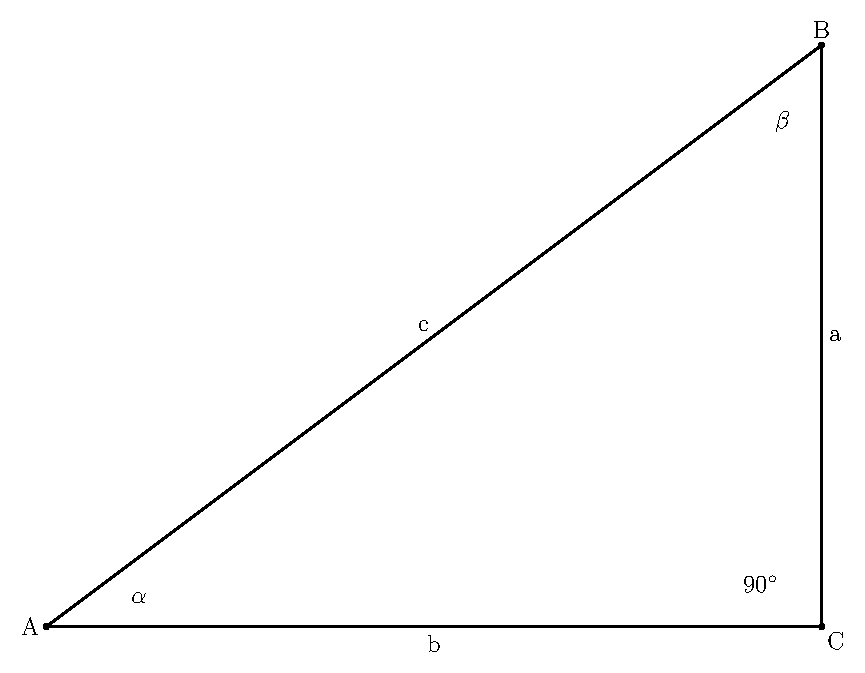
\includegraphics[scale=.3]{./right.eps}
  \end{figure}
\end{frame}

\begin{frame}
  \frametitle{Exercises}
{\ubung} Assume you know all the values of the cosine function for the interval
between $0^{\circ}$ and $90^{\circ}$. Evaluate the following expressions,
% 146 248 216 280 215  49 307 147 316 275
\begin{equation}
  \label{eq:reajoole}
  \sin\left(214^{\circ}\right)
\end{equation}
\begin{equation}
  \label{eq:poochail}
  \cot\left(146^{\circ}\right)
\end{equation}
\begin{equation}
  \label{eq:shiethei}
  \sin\left(248^{\circ}\right)
\end{equation}
\begin{equation}
  \label{eq:iejehies}
  \cos\left(216^{\circ}\right)
\end{equation}
\begin{equation}
  \label{eq:eefoghai}
  \tan\left(280^{\circ}\right)
\end{equation}
\begin{equation}
  \label{eq:aebeifii}
  \cos\left(307^{\circ}\right)
\end{equation}
\begin{equation}
  \label{eq:paeseing}
  \sin\left(49^{\circ}\right)
\end{equation}
\begin{equation}
  \label{eq:chaboong}
  \tan\left(147^{\circ}\right)
\end{equation}
\begin{equation}
  \label{eq:aewohnae}
  \tan\left(316^{\circ}\right)
\end{equation}
\end{frame}

\begin{frame}
  \frametitle{Exercises}
{\ubung} Solve the following equations for the given angle,
\begin{equation}
  \label{eq:yaezeiso}
  \sin\vartheta=\frac{1}{2},0^{\circ}\leq\vartheta\leq{}90^{\circ}
\end{equation}
\begin{equation}
  \label{eq:jaibiegi}
  \sin\vartheta=\frac{1}{2},90^{\circ}\leq\vartheta\leq{}180^{\circ}
\end{equation}
\begin{equation}
  \label{eq:puixifoh}
  \sin\vartheta=-\frac{1}{2},180^{\circ}\leq\vartheta\leq{}270^{\circ}
\end{equation}
\begin{equation}
  \label{eq:ieshokeo}
  \sin\vartheta=-\frac{1}{2},270^{\circ}\leq\vartheta\leq{}360^{\circ}
\end{equation}
\begin{equation}
  \label{eq:susoonou}
  \cos\vartheta=-\frac{1}{2},0^{\circ}\leq\vartheta\leq{}360^{\circ}
\end{equation}
\begin{equation}
  \label{eq:jooqueij}
  \tan\vartheta=1.9,0^{\circ}\leq\vartheta\leq{}360^{\circ}
\end{equation}
\end{frame}

\begin{frame}
  \frametitle{Exercises}
  {\ubung} Consider a right triangle with the length of the hypotenuse
  $c=10\sqrt{2}$ and the length of one side $a=8\sqrt{3}$. How long is
  the other side $b$? (Simplify the radical as in this example:
  $\sqrt{18}=3\sqrt{2}$.)
\end{frame}

\begin{frame}
  \frametitle{Exercises}
{\ubung} Express the following in terms of cosines of arguments between
$0^{\circ}$ and $90^{\circ}$.
\begin{equation}
  \label{eq:aleephua}
  \mbox{(a) }\sin\left(136^{\circ}\right)
\end{equation}
\begin{equation}
  \label{eq:ahghoome}
  \mbox{(a) }\tan\left(229^{\circ}\right)
\end{equation}
\begin{equation}
  \label{eq:ahgeefoo}
  \mbox{(a) }\cot\left(-171^{\circ}\right)
\end{equation}
\end{frame}

\begin{frame}
  \frametitle{Exercises}
  {\ubung} The sine of $54^{\circ}$ is
  $\frac{\sqrt{5}+1}{4}$. The sine of $30^{\circ}$ is $\frac{1}{2}$.
  Use this information to find the sine of $84^{\circ}$.
\end{frame}

\begin{frame}
  \frametitle{Exercises}
  {\ubung} What is the solution set for the following equation,
  $\cos\theta=\frac{\sqrt{3}}{2}$?
\end{frame}

\begin{frame}
  \frametitle{End of Lesson}
Next Lesson: Non-Right Triangles
\end{frame}

\end{document}
